\documentclass[11pt]{article}
\usepackage[a4paper,margin=1in]{geometry}
\usepackage{amsmath,amssymb,amsthm,mathtools,bm}
\usepackage{booktabs,tabularx,array}
\usepackage{graphicx}
\usepackage{xcolor}
\usepackage{microtype}
\usepackage{enumitem}
\usepackage{hyperref}
\usepackage[nameinlink,capitalise]{cleveref}

\hypersetup{
  colorlinks=true,
  linkcolor=blue!55!black,
  citecolor=blue!55!black,
  urlcolor=blue!55!black,
  pdftitle={Noisy Euclidean Correlators Do Not Certify a Spectral Gap Without Visibility},
  pdfauthor={Lluis Eriksson}
}

\newtheorem{theorem}{Theorem}[section]
\newtheorem{proposition}[theorem]{Proposition}
\newtheorem{corollary}[theorem]{Corollary}
\newtheorem{lemma}[theorem]{Lemma}
\theoremstyle{definition}
\newtheorem{definition}[theorem]{Definition}
\newtheorem{example}[theorem]{Example}
\theoremstyle{remark}
\newtheorem{remark}[theorem]{Remark}

\newcommand{\C}{\mathbb C}
\newcommand{\N}{\mathbb N}
\newcommand{\K}{\mathcal K}
\newcommand{\ran}{\operatorname{ran}}
\newcommand{\rank}{\operatorname{rank}}
\newcommand{\supp}{\operatorname{supp}}
\newcommand{\spec}{\operatorname{spec}}
\newcommand{\tr}{\operatorname{tr}}
\newcommand{\Id}{\mathbf 1}
\newcommand{\eps}{\varepsilon}

\title{\bfseries Noisy Euclidean Correlators Do Not Certify a Spectral Gap Without Visibility\\[3pt]
\large Hidden atoms, terminal moments, and multichannel witnesses}
\author{Lluis Eriksson}
\date{August 2026}

\begin{document}
\maketitle

\begin{abstract}
Euclidean correlation matrices are routinely converted into spectral gaps by
generalized eigenvalue, Prony, or Lanczos procedures.  We isolate a prior
question: when is a positive gap identifiable from a finite correlator window?
Let $T$ be a positive self-adjoint contraction and
$B_n=V^*T^nV$ its matrix-valued transfer moments.  The block Hankel pencil
$H_N=[B_{i+j}]$, $G_N=[B_{i+j+1}]$ gives monotone Ritz lower bounds on the
visible transfer edge.  Exact rank stabilization is terminal: it makes the
Krylov space invariant and recovers the entire visible spectrum after finitely
many moments.  Outside that singular regime we prove a finite-noise no-go.
For every normalized moment sequence and every $\eps>0$, mixing weight
$w\leq\eps$ with an atom at transfer eigenvalue one changes every moment by at
most $w$ while collapsing the mass lower bound to zero.  Thus no method can
uniformly certify a positive gap from finite moments with nonzero error without
a quantitative visibility assumption.  We then give a constructive converse.
If spectral mass at least $\gamma$ lies at least $\delta$ beyond a claimed edge
$\theta$, a degree-$N$ Chebyshev polynomial forces a negative Hausdorff
localizer once
\[
 \cosh^2\!\left(N\,\operatorname{arcosh}
 (1+2\delta/\theta)\right)>\theta/(\delta\gamma),
\]
with an explicit correction for componentwise moment error.  The filter is
minimax-optimal among degree-$N$ polynomials normalized at the resolved edge.
An interacting
ANNNI-chain experiment up to $2^{16}$ states exhibits the operational content:
a parity-even probe is exactly blind to the lowest odd excitation, while a
two-channel $(X,Z)$ family refutes a $35\%$ overstated gap at Krylov degree one
and recovers the transfer edge to $9.9\times10^{-5}$ at degree six.  Exact
rational certificates, the full numerical pipeline, a Colab notebook, and a
Lean-checked hidden-atom core are linked to fixed repository artifacts.
\end{abstract}

\section{The identifiability question}

A spectral gap is a support exclusion, not merely a fitted exponential slope.
In a transfer formulation, after removing the vacuum, it is the assertion
\begin{equation}
  \spec(T)\subset[0,e^{-m}]
  \qquad (m>0),                                      \label{eq:gap}
\end{equation}
for a positive self-adjoint contraction $T$.  Numerical and lattice
calculations generally do not access $T$ directly.  They access finitely many
matrices
\begin{equation}
  B_n=V^*T^nV,\qquad n=0,1,\ldots,M,                 \label{eq:moments}
\end{equation}
where the columns of $V:\C^d\to\K$ are states created by a chosen family of
interpolating operators.  These are Hausdorff moments of a positive
matrix-valued spectral measure.  This observation underlies generalized
eigenvalue methods, Prony-type reconstruction, Rayleigh--Ritz and block
Lanczos spectroscopy~\cite{Blossier2009,Fleming2023,Wagman2025,FilteredRR,MomentMatrix2025}.

The inverse problem has two logically different targets:
\begin{enumerate}[label=(\roman*)]
  \item estimate spectral values that are visible to the chosen probes;
  \item certify that no spectral value relevant to the claimed gap has been
  missed.
\end{enumerate}
The first is an approximation problem.  The second is an identifiability
problem.  A highly accurate estimate does not answer the second question if a
small spectral component can hide below the error floor.

This paper gives a three-branch answer.
\begin{description}
\item[Exact terminal branch.]
Rank stabilization of a block Hankel matrix is a finite, checkable condition
under which the Krylov approximation terminates and the visible spectrum is
recovered exactly.
\item[No-go branch.]
For every positive componentwise error radius, a spectral atom at transfer
eigenvalue one can be hidden inside the data ball.  No algorithm can infer a
uniform positive gap over the unconstrained model class.
\item[Visibility branch.]
A lower bound on the mass of any missed edge component turns the problem back
into a finite certificate.  A Chebyshev filter yields an explicit depth and
noise margin.
\end{description}

The algebraic ingredients are classical: positive moment problems,
Krylov termination, and Chebyshev acceleration.  The claim here is the
assembled operational boundary---including the impossibility theorem, the
minimal extra visibility datum, and an auditable correlator-only witness---not
the invention of Rayleigh--Ritz or of the truncated moment problem.

\section{Matrix moments and the visible spectral edge}

Let $\K$ be a complex Hilbert space, let $0\leq T\leq\Id$ be self-adjoint, and
let $V:\C^d\to\K$ be bounded.  Write $E_T$ for the spectral resolution of $T$
and
\begin{equation}
  \Sigma(A)=V^*E_T(A)V,
  \qquad B_n=\int_0^1 x^n\,d\Sigma(x)=V^*T^nV.       \label{eq:matrixmeasure}
\end{equation}
The visible cyclic subspace and its edge are
\begin{equation}
 \K_V=\overline{\operatorname{span}}\{T^j\ran V:j\geq0\},
 \qquad \rho_V=\|T|_{\K_V}\|.                       \label{eq:visibleedge}
\end{equation}
Only $T|_{\K_V}$ is identifiable from the moments.  If $\K_V\neq\K$, a
single probe family is blind to the orthogonal reducing complement.

For $N\geq0$ define block Hankel matrices
\begin{equation}
 H_N=[B_{i+j}]_{i,j=0}^N,qquad
 G_N=[B_{i+j+1}]_{i,j=0}^N.                          \label{eq:pencil}
\end{equation}
Given $c=(c_0,\ldots,c_N)\in(\C^d)^{N+1}$, set
\begin{equation}
 W_Nc=\sum_{j=0}^N T^jVc_j,
 \qquad q_c(x)=\sum_{j=0}^N x^jc_j.                  \label{eq:krylovmap}
\end{equation}
Then
\begin{align}
 c^*H_Nc&=\|W_Nc\|^2,\nonumber\\
 c^*G_Nc&=\langle W_Nc,TW_Nc\rangle,\nonumber\\
 c^*(\theta H_N-G_N)c
 &=\int_0^1(\theta-x)\,q_c(x)^*d\Sigma(x)q_c(x).     \label{eq:localizeridentity}
\end{align}

\begin{proposition}[Ritz/localizer dictionary]          \label{prop:ritz}
Let
\begin{equation}
 \rho_N=\sup_{c\notin\ker H_N}\frac{c^*G_Nc}{c^*H_Nc}.
\end{equation}
Then $\rho_N$ is the largest Ritz value of $T$ on
$\K_N=\ran W_N$, and
\begin{equation}
 0\leq\rho_N\leq\rho_{N+1}\leq\rho_V,
 \qquad \rho_N\uparrow\rho_V.                       \label{eq:ritzmonotone}
\end{equation}
Moreover, $\theta H_N-G_N\not\succeq0$ is a rigorous finite
falsifier of $\rho_V\leq\theta$, whereas
$\theta H_N-G_N\succeq0$ at one finite $N$ is not in general a certificate of
that support bound.
\end{proposition}

\begin{proof}
The first two identities in \cref{eq:localizeridentity} identify the
generalized Rayleigh quotient with that of $T$ on $\K_N$.  The inclusions
$\K_N\subseteq\K_{N+1}$ give monotonicity.  Their union is dense in $\K_V$,
so the variational suprema converge to $\|T|_{\K_V}\|$.  If a localizer has a
negative direction, \cref{eq:localizeridentity} is incompatible with spectral
support in $[0,\theta]$.  Positivity on polynomials of bounded degree does not
exclude spectral weight detectable only at larger degree.
\end{proof}

This proposition separates a common ambiguity.  A Ritz value is a lower bound
on the visible transfer edge and hence an \emph{upper} bound on the visible
mass $-\log\rho_V$.  A negative localizer falsifies an overstated mass.  Neither
becomes a full-gap theorem until probe completeness is supplied.

\section{The exact terminal branch}

Finite exact recovery occurs when the moment problem becomes degenerate.
This is the operator form of flat propagation in truncated moment theory and
of exact termination in block Lanczos~\cite{CurtoMatrix2022,CurtoExtremal2006,Madler2023,FilteredRR}.

\begin{theorem}[Flat Krylov termination]                \label{thm:flat}
If
\begin{equation}
  \rank H_N=\rank H_{N+1}<\infty,                      \label{eq:flat}
\end{equation}
then $\K_N=\K_{N+1}$, the space $\K_N$ is invariant under $T$, and
\begin{equation}
  \K_V=\K_N,qquad \rho_V=\rho_N.                      \label{eq:terminaledge}
\end{equation}
The finite generalized pencil $(G_N,H_N)$ on the quotient by $\ker H_N$
recovers the complete visible spectrum, with multiplicities in the cyclic
representation.  If in addition $\K_V=\K$, the recovered edge certifies the
full gap $m=-\log\rho_N$.
\end{theorem}

\begin{proof}
Since $H_N=W_N^*W_N$, $\rank H_N=\dim\K_N$.  The nesting
$\K_N\subseteq\K_{N+1}$ and \cref{eq:flat} therefore imply equality.  But
$T\K_N\subseteq\K_{N+1}$, hence $T\K_N\subseteq\K_N$.  All further Krylov
spaces equal $\K_N$, so their closure is $\K_V=\K_N$.  The compressed operator
is now the exact restriction rather than an approximation, and the quotient
pencil represents it in the nonorthogonal Krylov coordinates.
\end{proof}

\begin{example}[Exact rational terminal certificate]    \label{ex:rational}
Take
\[
 T=\operatorname{diag}(1/5,1/2,4/5),\qquad
 V=\begin{bmatrix}1&0\\1&1\\0&1\end{bmatrix}.
\]
The tracked exact-arithmetic artifact constructs $B_0,\ldots,B_5$ and finds
\[
 \rank H_0=2,\qquad \rank H_1=\rank H_2=3.
\]
On a rational quotient basis the pencil determinant is
\begin{equation}
 -\frac9{5000}(2\lambda-1)(5\lambda-4)(5\lambda-1),
\end{equation}
recovering $\{1/5,1/2,4/5\}$ exactly and hence the visible mass
$-\log(4/5)=\log(5/4)$.  No floating-point rank decision enters this example.
\end{example}

Flatness is powerful but singular.  With noisy data, exact rank is destroyed;
thresholding small singular values introduces a model choice.  The next
section shows that this is not merely a numerical inconvenience.

\section{A finite-noise no-go theorem}

The obstruction already appears for a scalar normalized spectral measure.
Its matrix analogue follows by adding an identity-valued atom.

\begin{theorem}[Hidden-atom indistinguishability]        \label{thm:nogo}
Let $\mu$ be a probability measure on $[0,1]$ with moments
$m_n=\int x^n\,d\mu(x)$.  For $0<w\leq1$ define
\begin{equation}
 \mu_w=(1-w)\mu+w\delta_1,
 \qquad m_n^{(w)}=(1-w)m_n+w.                          \label{eq:hiddenatom}
\end{equation}
Then, for every $n\geq0$,
\begin{equation}
  |m_n^{(w)}-m_n|=w(1-m_n)\leq w.                      \label{eq:hiddenbound}
\end{equation}
The measure $\mu_w$ has transfer edge one and therefore zero mass lower bound.
Consequently, for every finite window and every componentwise error radius
$\eps>0$, the error ball around the moments of a gapped measure contains the
moments of a zero-gap measure.

If $\Sigma$ is an $I_d$-normalized positive matrix measure and
$B_n=\int x^n d\Sigma(x)$, the same conclusion holds in operator norm for
\begin{equation}
 \Sigma_w=(1-w)\Sigma+w I_d\delta_1,
 \qquad B_n^{(w)}=(1-w)B_n+wI_d,
\end{equation}
because $0\preceq B_n\preceq I_d$ and
$\|B_n^{(w)}-B_n\|\leq w$.
\end{theorem}

\begin{proof}
Since $0\leq x^n\leq1$ on $[0,1]$, one has $0\leq m_n\leq1$.
Equation~\eqref{eq:hiddenbound} follows by direct subtraction.  The added atom
places positive spectral mass at $x=1$, so the support edge is one and
$-\log1=0$.  Choose any $w\leq\eps$.  The matrix statement is identical after
replacing scalar order by Loewner order.
\end{proof}

\begin{corollary}[Algorithm-independent impossibility]  \label{cor:algorithm}
No estimator whose only input is a finite positive-moment window with a
nonzero componentwise error bar can return a uniformly valid strictly positive
gap lower bound over all positive measures on $[0,1]$.
\end{corollary}

This conclusion applies equally to nonlinear fits, Bayesian reconstructions,
GEVP, Prony, Lanczos, Pad\'e, semidefinite programs, and machine-learning
estimators.  It is a property of the information set, not of the solver.  A
denoising projection onto the positive Hankel cone can improve consistency and
variance~\cite{Yu2024}; it cannot exclude the hidden measure in
\cref{thm:nogo} without adding a visibility prior.

The theorem is deliberately worst-case.  It does not say that small atoms are
common or that gap estimation is useless.  It says that a rigorous positive
certificate must disclose what rules them out.

\section{Visibility restores a finite certificate}

We now add exactly the missing quantitative datum.  Work first with a scalar
probability measure $\nu$ on $[0,1]$.  Fix a claimed edge
$0<\theta<1$, a resolution $0<\delta\leq1-\theta$, and a visibility floor
$0<\gamma\leq1$.

\begin{definition}[Visibility alternative]
The pair $(\delta,\gamma)$ is visible beyond $\theta$ if every admissible
measure whose edge reaches $\theta+\delta$ satisfies
\begin{equation}
 \nu([\theta+\delta,1])\geq\gamma.                    \label{eq:visibility}
\end{equation}
\end{definition}

The assumption is falsifiable and model-dependent.  It can come from a frame
bound for an operator family, a symmetry-resolved overlap estimate, a source
theorem, or an experimentally calibrated minimum spectral weight.  It cannot
be manufactured from the same noisy moments without circularity, by
\cref{thm:nogo}.

Let $\mathsf T_N$ denote the degree-$N$ Chebyshev polynomial of the first kind
and define
\begin{equation}
 p_N(x)=
 \frac{\mathsf T_N(2x/\theta-1)}
 {\mathsf T_N(1+2\delta/\theta)},
 \qquad
 \alpha_N=\frac1{\mathsf T_N(1+2\delta/\theta)}.       \label{eq:chebfilter}
\end{equation}

\begin{theorem}[Visibility-conditioned Chebyshev witness] \label{thm:cheb}
If \cref{eq:visibility} holds, then the degree-$N$ localizer value
\begin{equation}
 Q_N=\int_0^1(\theta-x)p_N(x)^2\,d\nu(x)              \label{eq:QN}
\end{equation}
satisfies
\begin{equation}
 Q_N\leq \theta\alpha_N^2-\delta\gamma.               \label{eq:Qbound}
\end{equation}
In particular $Q_N<0$, and the claimed support bound is falsified, whenever
\begin{equation}
 \cosh^2\!\left(N\operatorname{arcosh}
 (1+2\delta/\theta)\right)>
 \frac{\theta}{\delta\gamma}.                         \label{eq:depth}
\end{equation}
If $\delta\gamma<\theta$, it is sufficient that
\begin{equation}
 N>
 \frac{\operatorname{arcosh}\sqrt{\theta/(\delta\gamma)}}
 {\operatorname{arcosh}(1+2\delta/\theta)}.            \label{eq:Nexplicit}
\end{equation}
\end{theorem}

\begin{proof}
On $[0,\theta]$, the affine argument of $\mathsf T_N$ lies in $[-1,1]$,
so $|p_N|\leq\alpha_N$.  On $[\theta+\delta,1]$, the argument is at least
$1+2\delta/\theta$; monotonicity of $\mathsf T_N$ on $[1,\infty)$ gives
$p_N\geq1$.  Split \cref{eq:QN} into
$[0,\theta]$, $(\theta,\theta+\delta)$, and
$[\theta+\delta,1]$.  The three contributions are at most
$\theta\alpha_N^2$, $0$, and $-\delta\gamma$, respectively.  Finally use
$\mathsf T_N(y)=\cosh(N\operatorname{arcosh}y)$ for $y\geq1$.
\end{proof}

\begin{proposition}[Minimax stop-band leakage]           \label{prop:minimax}
Among all real polynomials $r$ of degree at most $N$ satisfying
$r(\theta+\delta)=1$, the smallest possible uniform leakage on the claimed
support is
\begin{equation}
 \inf_{\substack{\deg r\leq N\\r(\theta+\delta)=1}}
 \max_{0\leq x\leq\theta}|r(x)|
 =\frac1{\mathsf T_N(1+2\delta/\theta)}=\alpha_N.       \label{eq:minimax}
\end{equation}
The filter $p_N$ in \cref{eq:chebfilter} attains the infimum.
\end{proposition}

\begin{proof}
Under $y=2x/\theta-1$, the interval $[0,\theta]$ becomes $[-1,1]$ and the
normalization point becomes $y_0=1+2\delta/\theta>1$.  The Chebyshev extremal
property states that a degree-$N$ polynomial bounded by one on $[-1,1]$ has
absolute value at most $\mathsf T_N(y_0)$ at $y_0$.  Rescaling any candidate
$r$ therefore gives the lower bound in \cref{eq:minimax}.  The numerator of
$p_N$ has sup norm one on the interval and value
$\mathsf T_N(y_0)$ at the normalization point, so equality holds.
\end{proof}

Thus \cref{thm:cheb} uses the smallest possible uniform low-band amplitude for
its chosen degree and edge normalization.  This does not make
\cref{eq:depth} minimax over every conceivable nonlinear estimator or every
weighted error model; it establishes optimal separation within the polynomial
localizer class actually accessible from a finite moment window.

\begin{corollary}[Matrix-valued multichannel witness]    \label{cor:matrixcheb}
Let $\Sigma([0,1])=I_d$ and set
$\nu=d^{-1}\tr\Sigma$.  If
$\nu([\theta+\delta,1])\geq\gamma$ and \cref{eq:depth} holds, then
\begin{equation}
 \theta H_N-G_N\not\succeq0.
\end{equation}
Hence the matrix correlator window contains a finite direction that falsifies
the claimed edge.
\end{corollary}

\begin{proof}
Let $a_0,\ldots,a_N$ be the coefficients of $p_N$ and, for each standard basis
vector $e_\ell\in\C^d$, take the block coefficient vector
$c^{(\ell)}=(a_0e_\ell,\ldots,a_Ne_\ell)$.  Then
\[
 \frac1d\sum_{\ell=1}^d
 (c^{(\ell)})^*(\theta H_N-G_N)c^{(\ell)}=Q_N<0.
\]
At least one summand is negative.
\end{proof}

The degree grows only logarithmically with $1/\gamma$ at fixed resolution.
For small $\delta/\theta$, however,
$\operatorname{arcosh}(1+2\delta/\theta)\sim2\sqrt{\delta/\theta}$,
exposing the expected edge-resolution cost.  This is closely related to the
Chebyshev mechanism in Kaniel--Paige--Saad convergence bounds, but here the
output is a one-sided moment localizer with an explicit visibility premise,
not merely an eigenvalue convergence estimate~\cite{Saad1980,FilteredRR}.

\subsection{Certified moment error}

Write $p_N(x)=\sum_{j=0}^Na_jx^j$ and suppose measured moments satisfy
$|\widetilde m_k-m_k|\leq\eps$ for $0\leq k\leq2N+1$.  Form the measured
localizer $\widetilde Q_N$ by expanding \cref{eq:QN} in those moments.

\begin{proposition}[Noise-safe sign test]               \label{prop:noise}
The deterministic error obeys
\begin{equation}
 |\widetilde Q_N-Q_N|
 \leq(1+\theta)\eps\left(\sum_{j=0}^N|a_j|\right)^2
 =:R_N.                                                \label{eq:noiseradius}
\end{equation}
Therefore
\begin{equation}
 \widetilde Q_N+R_N<0                                 \label{eq:certsign}
\end{equation}
is a rigorous noisy-data falsifier of support in $[0,\theta]$.  Under the
visibility alternative, the sufficient worst-case condition
\begin{equation}
 \theta\alpha_N^2-\delta\gamma+R_N<0                  \label{eq:robustdepth}
\end{equation}
guarantees detection for every admissible error realization.
\end{proposition}

\begin{proof}
If $p_N^2=\sum_{k=0}^{2N}b_kx^k$, then
$Q_N=\theta\sum b_km_k-\sum b_km_{k+1}$.  Hence the error is at most
$(1+\theta)\eps\sum|b_k|$.  Convolution gives
$\sum|b_k|\leq(\sum|a_j|)^2$.  The sign and worst-case conclusions follow.
\end{proof}

Power-basis coefficients can grow rapidly.  Thus increasing $N$ is not
monotonically beneficial at fixed componentwise precision: spectral
localization improves while the rigorous error radius may worsen.  The tracked
stress test with $\theta=0.8$, $\delta=0.1$, $\gamma=10^{-2}$ and
$\eps=10^{-14}$ becomes negative at degree five; the analytic sufficient bound
turns negative at degree six.  Higher precision or a stable recurrence-based
error model can extend the useful window, but must be declared explicitly.

\section{Interacting spin-chain test}

Theorems about visibility should be tested in a model where blindness is exact
and the transfer operator is not inserted by hand.  We use the open quantum
ANNNI chain
\begin{equation}
 H_L=-J_1\sum_{j=1}^{L-1}Z_jZ_{j+1}
     -J_2\sum_{j=1}^{L-2}Z_jZ_{j+2}
     -h_x\sum_{j=1}^{L}X_j,                            \label{eq:annni}
\end{equation}
at $(J_1,J_2,h_x)=(1,0.37,2.2)$.  This generic next-nearest-neighbour
interacting instance is not treated through a free-fermion solution.  It
preserves the global parity $P=\prod_jX_j$.  The computed ground state is even
and the first excited state odd throughout $L=6,8,\ldots,16$.

Let $|0\rangle$ be the independently computed ground state and, at the central
site, define centered probes
\begin{equation}
 |\psi_X\rangle=(X_c-\langle X_c\rangle)|0\rangle,
 \qquad
 |\psi_Z\rangle=(Z_c-\langle Z_c\rangle)|0\rangle.     \label{eq:probes}
\end{equation}
Because $X_c$ is parity even, its overlap with the first odd state vanishes
exactly.  Because $Z_c$ is odd, it can see that state.  With $\tau=0.2$ we
construct only the correlator matrices
\begin{equation}
 B_n^{ab}=\langle\psi_a|
 e^{-n\tau(H_L-E_0)}|\psi_b\rangle,
 \qquad a,b\in\{X,Z\}.                                \label{eq:annnimoments}
\end{equation}
The moment pipeline is then separated from the low-energy diagonalization used
as ground truth.

\begin{figure}[t]
 \centering
 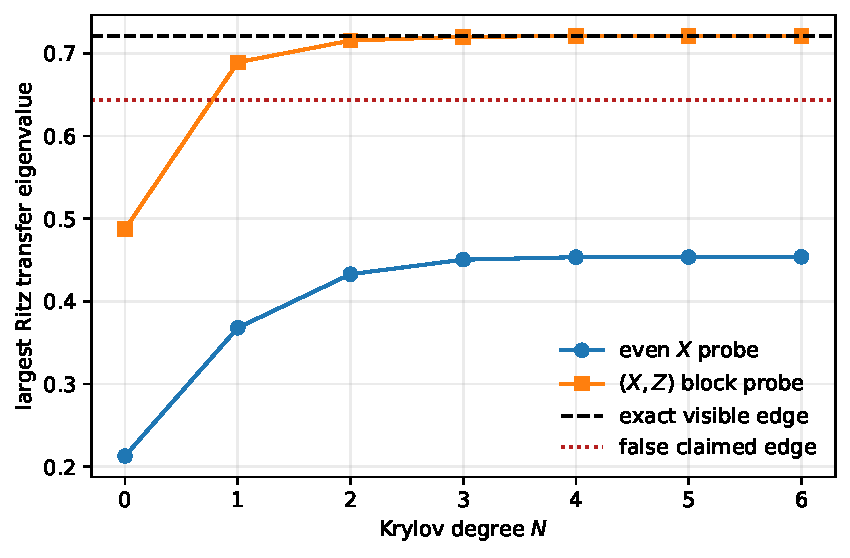
\includegraphics[width=.78\linewidth]{../../verification/finite_window_gap_certificates/figures/annni_ritz_convergence.pdf}
 \caption{Largest Ritz transfer value for $L=12$.  The even $X$ probe
 converges to the lowest visible even excitation and misses the true edge.  The
 $(X,Z)$ block family converges rapidly to the exact edge.}
 \label{fig:ritz}
\end{figure}

\begin{figure}[t]
 \centering
 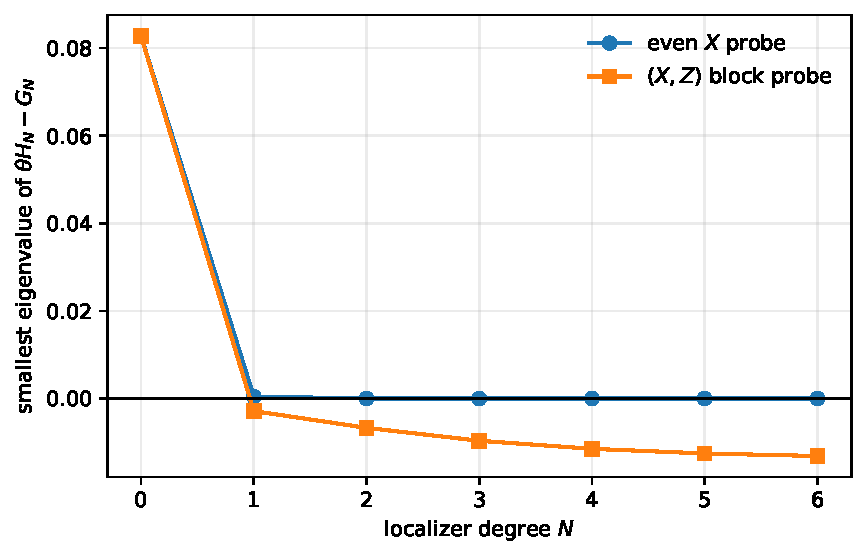
\includegraphics[width=.78\linewidth]{../../verification/finite_window_gap_certificates/figures/annni_localizer_witness.pdf}
 \caption{Smallest eigenvalue of the localizer for a gap overstated by
 $35\%$.  The multichannel family gives a negative certificate from degree one;
 the symmetry-blind $X$ family never does.}
 \label{fig:localizer}
\end{figure}

\Cref{fig:ritz,fig:localizer} show the two distinct outputs.  The Ritz value
estimates an edge; the negative localizer certifies that a proposed smaller
edge is impossible for the measured spectral measure.  The single even probe
can look numerically stable while converging to the wrong sector.

\begin{table}[t]
\centering
\small
\caption{ANNNI scaling.  $w_X,w_Z$ are squared overlaps with the first excited
state.  $\widehat\rho_6$ is the block-Krylov edge from moments through order 13.
All rows refute the $35\%$ overstated gap at degree one; the $X$-only family
never refutes it through degree six.}
\label{tab:annni}
\begin{tabular}{rrrrrr}
\toprule
$L$ & $E_1-E_0$ & $\rho=e^{-.2(E_1-E_0)}$ & $w_X$ & $w_Z$ &
$|\widehat\rho_6-\rho|$\\
\midrule
6  & 2.0845863 & 0.6590755 & $3.4\,10^{-31}$ & 0.45160 & $1.9\,10^{-7}$\\
8  & 1.8574804 & 0.6897017 & $4.3\,10^{-32}$ & 0.39733 & $3.9\,10^{-6}$\\
10 & 1.7217194 & 0.7086852 & $9.8\,10^{-34}$ & 0.35390 & $2.1\,10^{-5}$\\
12 & 1.6335802 & 0.7212885 & $2.0\,10^{-32}$ & 0.31837 & $5.7\,10^{-5}$\\
14 & 1.5729200 & 0.7300925 & $2.8\,10^{-30}$ & 0.28900 & $8.6\,10^{-5}$\\
16 & 1.5293122 & 0.7364879 & $1.2\,10^{-31}$ & 0.26437 & $9.9\,10^{-5}$\\
\bottomrule
\end{tabular}
\end{table}

\begin{figure}[t]
 \centering
 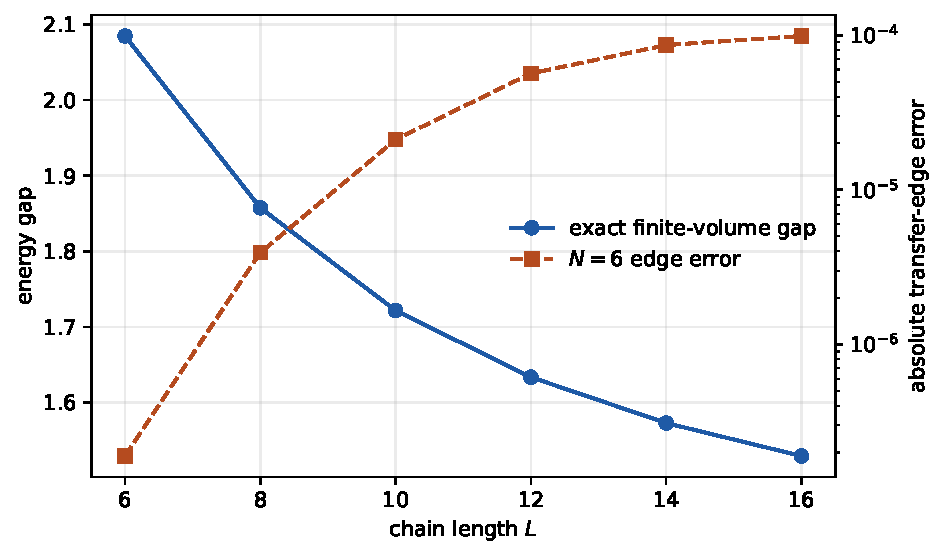
\includegraphics[width=.78\linewidth]{../../verification/finite_window_gap_certificates/figures/annni_scaling.pdf}
 \caption{Independent finite-volume energy gap and degree-six transfer-edge
 error.  The $L=12,14,16$ run was executed in Colab Pro+ on the fixed source
 commit recorded in the artifact.  This is a finite-size validation, not a
 thermodynamic-gap extrapolation.}
 \label{fig:scaling}
\end{figure}

At $L=16$ the Hilbert-space dimension is $65{,}536$.  The independent gap is
$1.5293121573$, the true transfer edge is $0.7364879301$, and the degree-six
block value is $0.7363890221$.  Its absolute error is
$9.89\times10^{-5}$.  The first-state weights are
$w_X=1.17\times10^{-31}$ and $w_Z=0.26437$.  These numbers do not prove a
thermodynamic mass gap; they validate the visibility mechanism and the
correlator-only certificate at nontrivial finite size.

\section{Reproducibility and formal boundary}

All computational claims are generated from public, deterministic artifacts:
\begin{itemize}
  \item exact rational flat-extension, hidden-atom, and Chebyshev artifacts;
  \item sparse ANNNI construction, independent low-energy benchmark, moment
  construction, block pencils, and localizers;
  \item tracked local JSON for $L=6,8,10,12$;
  \item a Colab summary for $L=12,14,16$, including Python/NumPy/SciPy
  versions, source commit, and full-result SHA-256;
  \item scripts that regenerate all three figures.
\end{itemize}
Running the tracked \texttt{verify\_all.py} from the repository root
regenerates the exact artifact and audits every theorem-level invariant quoted
from the local and Colab records; its README gives the one-line command.
The verification directory is
\href{https://github.com/lluiseriksson/aqft-split-inclusion-series/tree/agent/positive-spectral-resource-boundaries/verification/finite_window_gap_certificates}
{publicly archived in the companion repository}.
The Colab entry point is
\href{https://github.com/lluiseriksson/aqft-split-inclusion-series/blob/agent/positive-spectral-resource-boundaries/verification/finite_window_gap_certificates/colab_annni_scale.ipynb}
{\texttt{colab\_annni\_scale.ipynb}}.

The algebraic core of \cref{thm:nogo} is separately formalized in Lean 4 at
fixed commit
\href{https://github.com/lluiseriksson/lean-transfer-matrix/blob/1e41144/LeanTransferMatrix/FiniteNoiseBlindness.lean}
{fixed Lean source}, with the
\href{https://github.com/lluiseriksson/lean-transfer-matrix/blob/1e41144/audit/FiniteNoiseBlindnessAxioms.lean}
{axiom audit} and
\href{https://github.com/lluiseriksson/lean-transfer-matrix/pull/25}
{draft PR \#25}.  The build checks 8,158 targets with no \texttt{sorry} and no
project axioms.  The reported theorem dependencies are exactly
\{\texttt{propext}, \texttt{Classical.choice}, \texttt{Quot.sound}\}.

The formalization proves the normalized hidden-atom mixture, componentwise
distance bound, preservation of the interval constraints, existence inside
every error ball $0\leq\eps\leq1$, and $-\log1=0$.  It does not formalize the
spectral theorem, Chebyshev integral bound, or ANNNI numerics.  Those remain
paper proofs and reproducible computations, respectively.

\section{Relation to prior methods and novelty audit}

Matrix Euclidean correlators as moment data, their relation to
Rayleigh--Ritz/Lanczos, and rigorous bounds on smeared spectral functions are
developed in~\cite{MomentMatrix2025}.  The Prony--Ritz equivalence class and
exact solution of finite-dimensional spectra from sufficient correlation data
are analysed in~\cite{FilteredRR}; matrix-polynomial combinations of GEVP and
Prony appear in~\cite{Fleming2023}.  GEVP convergence with increasing operator
bases is classical in lattice spectroscopy~\cite{Blossier2009}, and direct
imaginary-time gap estimators have been tested in many-body models
in~\cite{Leamer2023}.  Recursive and flat matrix moment problems are studied in
\cite{CurtoMatrix2022,CurtoExtremal2006,Madler2023}.  None of those facts is
claimed as new here.

\begin{table}[ht]
\centering
\small
\caption{Claim audit.  ``This paper'' means the stated combination and
specialization, not ownership of the classical ingredients.}
\begin{tabularx}{\linewidth}{>{\raggedright\arraybackslash}p{.28\linewidth}
>{\raggedright\arraybackslash}p{.32\linewidth}X}
\toprule
Item & Prior status & Contribution here\\
\midrule
Matrix moments and block Ritz & Established in moment and lattice spectroscopy
& Unified notation tied to a one-sided gap localizer\\
Exact finite recovery & Standard Krylov termination/flat moment phenomenon
& Checkable terminal criterion stated directly for visible transfer gaps and
verified by an exact rational artifact\\
Finite-noise hidden edge & Elementary mixture mechanism; small-component
instability is familiar in inverse problems
& Algorithm-independent zero-gap construction inside every positive moment
error ball, with a matrix version and Lean-checked core\\
Minimum visibility & Minimum amplitude assumptions occur in support recovery
& Identified as the missing datum for rigorous gap certification, rather than
an optional numerical regularizer\\
Chebyshev filtering & Classical in extremal eigenvalue convergence
& Explicit localizer sign theorem with $(\theta,\delta,\gamma,N)$ depth and a
componentwise error radius, plus minimax optimality of its uniform stop-band
leakage among normalized degree-$N$ polynomial filters\\
Probe blindness & Symmetry selection rules are standard
& Controlled interacting example separating a stable wrong-sector estimate
from a multichannel finite certificate through $2^{16}$ states\\
\bottomrule
\end{tabularx}
\end{table}

The main conceptual advance is therefore a boundary theorem: finite noisy
correlators support rigorous gap falsification, and under disclosed visibility
they support finite detection, but they do not support an unconditional
positive gap certificate.  Exact flatness is the exceptional terminal regime.

\section{Consequences and limitations}

\paragraph{For lattice mass-gap programmes.}
A finite correlator analysis can disprove an overstated transfer gap by a
negative localizer.  To prove a positive volume-uniform gap, one still needs a
volume-uniform totality or visibility theorem for the chosen gauge-invariant
operator family, controlled errors, and the reconstruction connecting the
Euclidean measure to a positive transfer operator.  The present results do not
establish any of those model-dependent inputs for four-dimensional
Yang--Mills.

\paragraph{For operator design.}
Adding channels is not merely a variance-reduction strategy.  It changes the
visible cyclic subspace.  Symmetry-resolved operator families should be judged
by quantitative frame or overlap bounds, not only by the apparent stability of
their extracted levels.

\paragraph{For noisy moment algorithms.}
Projection to the positive Hankel cone is useful for restoring consistency,
but a projected point estimate should not be reported as a support theorem.
The visibility floor and the propagated sign margin in
\cref{eq:certsign} are the appropriate certificate metadata.

\paragraph{Limitations.}
The Chebyshev stop-band factor is minimax optimal only within normalized
degree-$N$ scalar polynomial filters; the resulting mass-versus-leakage sign
condition is sufficient, not a necessary identifiability threshold.  The
componentwise error model ignores correlations and can be conservative.  The
ANNNI study is finite-volume and uses exact sparse propagation rather than
Monte Carlo data.  No thermodynamic extrapolation is attempted.  Matrix-valued
optimal filters, correlated confidence regions, interval arithmetic, and
formalization of the Chebyshev theorem remain open extensions.

\section{Conclusion}

The distinction between estimating a visible level and certifying a spectral
gap is structural.  Block Hankel pencils give monotone visible-edge estimates
and finite falsifiers.  Exact rank stabilization closes the problem at finite
depth.  With any nonzero error and no visibility premise, however, a hidden
atom at transfer eigenvalue one lies inside the data ball and destroys every
uniform positive gap conclusion.  A quantitative visibility floor is the
minimal bridge back to a finite theorem; Chebyshev localization makes its cost
explicit.  The interacting spin-chain test shows why this distinction matters:
a symmetry-blind probe can converge smoothly and still miss the gap-controlling
state, while a multichannel family supplies an immediate negative witness.

\begin{thebibliography}{99}

\bibitem{Blossier2009}
B.~Blossier, M.~Della Morte, G.~von Hippel, T.~Mendes, and R.~Sommer,
``On the generalized eigenvalue method for energies and matrix elements in
lattice field theory,'' \emph{JHEP} \textbf{04}, 094 (2009),
\href{https://arxiv.org/abs/0902.1265}{arXiv:0902.1265}.

\bibitem{Fleming2023}
G.~T.~Fleming, ``Beyond generalized eigenvalues in lattice quantum field
theory'' (2023),
\href{https://arxiv.org/abs/2309.05111}{arXiv:2309.05111}.

\bibitem{Wagman2025}
M.~L.~Wagman, ``Lanczos, the transfer matrix, and the signal-to-noise
problem,'' \emph{Phys. Rev. Lett.} \textbf{134}, 241901 (2025),
\href{https://arxiv.org/abs/2406.20009}{arXiv:2406.20009}.

\bibitem{FilteredRR}
R.~Abbott, D.~C.~Hackett, G.~T.~Fleming, D.~A.~Pefkou, and M.~L.~Wagman,
``Filtered Rayleigh--Ritz is all you need'' (2025),
\href{https://arxiv.org/abs/2503.17357}{arXiv:2503.17357}.

\bibitem{MomentMatrix2025}
R.~Abbott, W.~I.~Jay, and P.~R.~Oare,
``Moment problems and bounds for matrix-valued smeared spectral functions''
(2025), \href{https://arxiv.org/abs/2508.01377}{arXiv:2508.01377}.

\bibitem{Leamer2023}
J.~M.~Leamer, A.~B.~Magann, G.~McCaul, and D.~I.~Bondar,
``Spectral gaps via imaginary time'' (2026),
\href{https://arxiv.org/abs/2303.02124}{arXiv:2303.02124}.

\bibitem{Yu2024}
Y.~Yu, A.~F.~Kemper, C.~Yang, and E.~Gull,
``Denoising of imaginary time response functions with Hankel projections,''
\emph{Phys. Rev. Research} \textbf{6}, L032042 (2024),
\href{https://arxiv.org/abs/2403.12349}{arXiv:2403.12349}.

\bibitem{CurtoMatrix2022}
R.~Curto, A.~Ech-charyfy, K.~Idrissi, and E.~H.~Zerouali,
``A recursive approach to the matrix moment problem'' (2023),
\href{https://arxiv.org/abs/2209.01630}{arXiv:2209.01630}.

\bibitem{CurtoExtremal2006}
R.~E.~Curto, L.~A.~Fialkow, and H.~M.~M\"oller,
``The extremal truncated moment problem,''
\href{https://arxiv.org/abs/math/0610882}{arXiv:math/0610882}.

\bibitem{Madler2023}
C.~M\"adler and K.~Schm\"udgen,
``On the truncated matricial moment problem. I'' (2023),
\href{https://arxiv.org/abs/2310.00957}{arXiv:2310.00957}.

\bibitem{Saad1980}
Y.~Saad, ``On the rates of convergence of the Lanczos and the block-Lanczos
methods,'' \emph{SIAM J. Numer. Anal.} \textbf{17}, 687--706 (1980).

\bibitem{Luscher1977}
M.~L\"uscher, ``Construction of a selfadjoint, strictly positive transfer
matrix for Euclidean lattice gauge theories,'' \emph{Commun. Math. Phys.}
\textbf{54}, 283--292 (1977).

\end{thebibliography}

\end{document}
